% literature review

\section{Introduction}

Earlier it was stated that sharing tacit knowledge requires relatively high levels of motivation and trust. It is also about empowering others to perform their work. This chapter considers theories of motivation, trust, and power. The goal is to come up with a conceptual framework for analysing tacit knowledge sharing behaviour.

\section{On the nature of knowledge}

Before delving into the theories of motivation, trust, and power, it is important to first clarify what knowledge is and understand what knowledge management is about. Knowledge is defined as information that is \enquote{relevant, actionable, and at least partially based on experience. experience. Knowledge is a subset of information, is subjective, is linked to meaningful behaviour, and it has tacit elements born of experience} \citep{leonard1998role}. This definition assumes knowledge ranges from being almost completely tacit, embodied in individual and group practice, to almost completely explicit, accessible to others in a codified and structured form \citep{polanyi1966tacit,nelson1982evolutionary,inkpen1998knowledge,leonard1998role,munoz2015tacit}. \medskip

A primary challenge in knowledge management is translating individual or group learning into organisational capability \citep{hansen2005share,lam2010knowledge,girard2015defining}. Unless a person or a group decides to share their knowledge, it remains a hidden and untapped resource \citep{davenport1998working}. Knowledge sharing can be understood as the behaviour by which an individual or group voluntarily provides others with access to their unique knowledge and experiences \citep{cabrera2002knowledge,hansen2005share}. Understanding what motivates people to share their knowledge is central to this study. \medskip

\section{Motivation}

Motivation is a theoretical construct used to explain individual behaviour. A motive is what prompts a person to act in a certain way, or at least develop an inclination for specific behaviour \citep{pardee1990motivation}. \medskip

\subsection{Self-efficacy}

\citet{white1959motivation} argues individual behaviour is mostly driven by an innate desire to become more competent in dealing with the environment. According to him, motivation is about achieving a greater sense of self-efficacy or behavioural control over the environment. \citet{bandura1977self} posits that individuals develop self-efficacy through modelling human behaviour. By observing others, an individual can see how patterns of behaviour are performed, which then serves as a guide for future action. Feedback received after taking action helps the individual adjust or self-correct their behaviour. In this way, an individual is able to develop a stronger sense of self-efficacy \citep{bandura1977self}. \medskip

As mentioned earlier, tacit knowledge is not transferred but rather interpreted within a specific context \citep{nonaka1995knowledge,duguid2005art,marabelli2014knowing}. Face-to-face social interaction is considered the richest medium because it allows immediate feedback to check understanding and correct interpretations \citep{koskinen2003tacit}. From this, we can postulate that acquiring tacit knowledge satisfies a desire to feel competent. \medskip

High self-efficacy can affect motivation in both positive and negative ways. People with high self-efficacy are more likely make efforts to complete a task, and to persist longer in those efforts, than those with low self-efficacy \citep{schunk1990goal}. Challenges often stimulate people with high self-efficacy to greater efforts, whereas someone with low self-efficacy will tend toward discouragement and giving up \citep{zimmerman1992self}. From this we can postulate people with higher levels of self-efficacy will be inclined to be more innovative \citep{gist1989influence}. \medskip 

\emph{Proposition 1: People with higher-levels of self-efficacy are more likely to seek out tacit knowledge and generate new ideas.}

\subsection{Theory of planned behaviour}

The theory of planned behaviour suggests actions and behaviours reliably follow intentions \citep{ajzen1985intentions}. Intentions capture the motivational factors that influence a particular behaviour. The theory of planned behaviour postulates three conceptually independent determinants of intention: First, is \emph{attitude} toward the behaviour and refers to the degree to which a person has a favourable or unfavourable disposition to the behaviour in question. Second, is \emph{subjective norm} that refers to the perceived social pressure to perform or not to perform the behaviour. Third, is the degree of perceived behavioural control or \emp{self-efficacy}, which as stated earlier, refers to how people rate their ability to succeed in specific situations or accomplish a task \citep{bandura1982self,ajzen1991theory}. The theory of planned behaviour suggests that the motivation to share knowledge is dependent not just on perceived self-efficacy, but also on personal attitudes and subjective norms. \medskip

\subsection{Self-determination theory}

Self-determination theory suggests humans are innately driven to seek out competence, autonomy and relatedness \citep{ryan2000self}. The theory distinguishes between controlled and autonomous motivation. Being controlled involves acting under some sense of pressure. Autonomy involves acting with a sense of volition and having the experience of choice. \medskip

Intrinsically motivated behaviour is driven by an individual’s interest or pleasure in the activity itself. Such behaviour is essentially autonomous. Less interesting activities require extrinsic motivation, where people's actions depend on the perceived contingency between behaviour and the desire for implicit approval or tangible rewards \citep{gagne2005self}. Extrinsic motivation can vary in the degree to which it is autonomous or controlled. Externally regulated behaviour is a form of controlled motivation. Other types of extrinsic motivation result when behavioural regulation is internalised. Regulation that has been taken in by a person but is not accepted as their own is said to be introjected. Such regulation may be seen as a form of internalised extrinsic motivation. With identified regulation, people feel a greater sense of autonomy because their behaviour is aligned to their personal goals and identities \citep{gagne2005self}. \medskip

The primary difference between self-determination theory and other work motivation theories is that self-determination theory focuses on the relative strength of autonomous versus controlled motivation rather than on the total amount of motivation. Research indicates that autonomous motivation facilitates effective performance and well-being, whereas controlled motivation can detract from those outcomes, particularly if the task requires creativity, cognitive flexibility, or deep processing of information \citep{gagne2005self}. This is particularly salient for innovation. \medskip

Self-determination theory can help explain individual motivation to share knowledge \citep{gagne2009model}. As long as knowledge sharing is voluntary, sharing parties tend to perceive it as intrinsically satisfying because it is self-determined and enhances their sense of self-worth and competence \citep{kaser2001knowledge,lam2010knowledge,dumbach2014establishing}. Moreover, since knowledge sharing is a social act, it is able to satisfy an individual's need for relatedness \citep{llopis2016understanding}. Autonomously motivated people will have greater belief in their own ability to accomplish tasks (higher level of self-efficacy). Such people are more inclined to take on challenging tasks and learn from these \citep{bandura1977self}. Consequently, people who are autonomously motivated are likely accumulate more tacit knowledge compared to those inclined towards controlled motivation. \medskip

\emph{Proposition 2: People with higher levels of autonomous motivation are more likely to seek out tacit knowledge from experienced others}


\citet{deci1985general} distinguish between intrinsic motivation, which refers to doing something because it is inherently interesting or enjoyable, and extrinsic motivation, which refers to doing something because it leads to a separable outcome. 

\section{Cognitive evaluation theory}

Cognitive evaluation theory is a sub-theory of self-determination theory that focuses on competence and autonomy while examining how intrinsic motivation is affected by external forces. The primary implication for cognitive evaluation theory is that the consequences of a reward will be a decreased level of intrinsic motivation and satisfaction because the reward is perceived to negatively impact the autonomy and competence of the individual \citep{deci1999meta}. 

Past studies have looked at how firms can motivate people to share knowledge \citep[e.g.][]{cabrera2002knowledge,ipe2003knowledge,cabrera2006determinants,wang2010knowledge,witherspoon2013antecedents,von2015s}. \citet{ipe2003knowledge} refers to internal and external factors that influence the motivation to share knowledge. Internal factors include the perceived power attached to the knowledge and reciprocity that results from sharing. External factors include the relationship with the recipient and rewards for sharing \citep{ipe2003knowledge}. \medskip

The accumulation of tacit knowledge requires considerable investment of time and resources. Those who have invested heavily in their current knowledge may not be willing to unlearn. Long-held views and knowledge acquired and reinforced over a long period of time may be considered more difficult to unlearn than recently acquired knowledge, to which the individual has less of an emotional attachment \citep{rebernik2007fostering}. \medskip

\section{Trust}

Trust is at the heart of knowledge exchange \citep{davenport1998working}. An open innovation initiative is unlikely to succeed if trust between partners is lacking. Partners are expected to share their skills, expertise and competencies for mutual benefit. Higher levels of trust are believed to lead to more effective collaboration \citep{axelrod1984evolution}. Trust limits opportunistic behaviour, builds commitment, and creates a safe environment to resolve issues \citep{panteli2005trust}. \medskip

Trust may be characterised as \enquote{the willingness of a party to be vulnerable} \citep{mayer1995integrative}. \citet{rousseau1998not} define trust as \enquote{a psychological state comprising the intention to accept vulnerability based upon positive expectations of the intentions or behaviour of another}. Trust may be inter-personal or inter-organisational in nature \citep{zaheer1998does}. Inter-personal trust is about the positive expectation a person has of the behaviour of someone else, whereas inter-organisational trust is more about confidence in an organisation's reliability and integrity \citep{ashnai2016inter}. Inter-personal trust feeds inter-organisational trust. Higher levels of inter-organisational trust can help reduce conflict and transaction costs \citep{zaheer1998does}. \medskip 

When trust exists, people are more willing to share their knowledge and be receptive of other people's knowledge \citep{levin2004strength}. People who have invested a lifetime building their tacit knowledge are unlikely to give up control over their personal knowledge if this makes them feel more vulnerable \citep{leonard1998role,lin2007share}. The management challenge is to create a safe environment that allows individuals to share their tacit knowledge in ways that will not deprive them control of this very personal knowledge \citep{bordum2002tacit}. \medskip

Trust is a dynamic phenomenon, changing with the passage of time as individuals learn about one another \citep{blomqvist1997many,panteli2005trust}. Though trust is seen as something that builds incrementally and accumulates over time, open innovation demands a more short-term view of trust. Each collaboration may be seen as a \enquote{temporary} or \enquote{virtual} organisation established to deliver a specific innovation within a market-relevant time-frame \citep{cococcioni2014exploring}. Time is a vital but often elusive component in the trust-building process \citep{kasper2001communicating}. Swift trust is a form of trust occurring in temporary organisations. Such trust is particularly important in temporary organisations because it substitutes the traditional mechanisms of control and coordination found in established hierarchies \citep{kasper2001communicating}. Trust is initially assumed by members of a temporary organisations but adjust their trust beliefs on the basis of fulfilled or unfulfilled expectations.

% This requires a good approach to conflict management. Effective conflict management enhances the trust development process and enables partners to be more open in the level and nature of knowledge shared, debate and challenge engaged in, and thus more capable of learning and knowledge creation \citep{panteli2005trust}. \medskip

Trust is cognition-based insofar as \enquote{we choose whom we will trust in which respects and under what circumstances, and we base the choice on what we take to be \enquote{good reasons}, constituting evidence of trustworthiness} \citep{lewis1985trust}. From this, one can say that cognition-based trust is largely self-determined. Emotional ties linking individuals provide the basis for affect-based trust \citep{mcallister1995affect}. Affect-based trust has a significantly greater effect on willingness to \emph{share} tacit knowledge, whereas cognition-based trust plays a greater role in willingness to \emph{use} tacit knowledge \citep{levin2004strength,holste2010trust}. \medskip

Trust in knowledge sharing networks may be indicated by reciprocity or transitive or path closure. Reciprocity is a key concept in social exchange and game theory and reflects a human tendency to return helpful or harmful acts in kind  \citep{nowak2005evolution}. Social exchange theory assumes actors enter into social relations to obtain some desired goal or reward \citep{homans1961social,blau1964exchange}. Actors consciously or sub-consciously use cost-benefit analysis to optimise their social interactions so that rewards outweigh costs. Reciprocity can be direct (\enquote{you scratch my back, and I will scratch yours}) or indirect (\enquote{I will give you advice, if you buy me a coffee}).  


Reciprocation is less likely if costs are too high. Exchanges can be characterised in terms of behavioural or relational responses. A positive initiating action would increase trust, a type of relational response, which in turn would promote a positive behavioural response \citep{cropanzano2016social}. 

Game theory attempts to explain the interaction people have with one another. It was originally conceived as an economic and mathematical theory that predicted that human interaction had the characteristics of a game, including strategies, winners and losers, rewards and punishment, and profits and cost \citep{axel}. 


Put simply, reciprocity helps build trust and strengthen ties between actors \citep{blau1964exchange}. 


This is especially true with respect to tacit knowledge sharing, which takes significant effort to communicate.  . Unequal exchanges lead to a power imbalances. 

One can surmise that unless tacit knowledge sharing is reciprocated, people may feel they are losing control over their personal knowledge and will stop being so trusting of others with regard to their tacit knowledge. \medskip


Exchanges entail some cost to the actor in terms of time, energy, and resources.


. Transitive or path closure is a form of implicit trust. Path closure  - \enquote{a friend of a friend, is a friend of mine}). 



\medskip


% build trust, brokers, recip, closure

% \begin{table}[]
% \centering
% \caption{Summary of the concepts commonly used as synonyms of trust \citep{blomqvist1997many}.}
% \label{trust}
% \begin{tabular}{@{}lll@{}}
% \toprule
% Concept & Definition & Connection to trust \\ \midrule
% Competence & The actor's perceived ability to perform something. & A passive concept describing an actor's ability to perform. \\
% Credibility & The actor's perceived ability to perform something he claims he can do on request. & A passive concept referring to the actor's claimed ability, which does not however say anything about the actor's intentions nor his will to do the requested. \\
% Confidence & The actor expects something to happen with certainty, and does not consider the possibility of anything going wrong. & Does not involve the conscious consideration of alternatives, as trust does. \\
% Faith & Actor's blind belief in something. & The actor does not have, or does not request information for considering alternatives as in the case of trust does. \\
% Hope & The actor passively looks forward to something. & Due to the actor's passivity he or she does not invest/risk anything by hoping, in the case of trusting. \\
% Loyalty & The actor has taken a faithful stand relative to another actor, behaving totally positively towards that actor's needs. & A static and long-term concept, does not seem to involve the possibility of breaking down. \\
% Reliance & The actor may on consideration decide to rely only on certain aspects or features of another actor or system. & A narrower concept than trust in the sense that a trusting actor trusts another in all respects after judging the character and behaviour of the other. \\ \bottomrule
% \end{tabular}
% \end{table}


From a network perspective, trust , 


\subsection{Social exchange theory}

 

%\begin{table}[]
%\centering
%\caption{Conditions of exchange. From \citet{blau1964exchange}.}
%\label{socextheory}
%\begin{tabular}{@{}llll@{}}
%\toprule
% & \multicolumn{1}{c}{\textbf{Intrinsic}} & %\multicolumn{1}{c}{\textbf{Extrinsic}} & %\multicolumn{1}{c}{\textbf{Unilateral}} \\ \midrule
%\textbf{Spontaneous evaluations} & Personal attraction %& Social approval & Respect - Prestige \\
%\textbf{Calculated actions} & Social acceptance & %Instrumental services & Compliance - Power \\ %\bottomrule
%\end{tabular}
%\end{table}


\emph{Proposition 3: Actors are more likely to seek tacit knowledge from others with know-how gained through experience.}





Past studies emphasise the importance of strong ties for communicating knowledge \citep[e.g.][]{hansen1999search,szulanski1996exploring,uzzi1997social}.







\section{Power}

The power literature is dominated by two contrasting views of power: \enquote{power as domination}, also referred to as \enquote{power-over}, and \enquote{power as empowerment}, often characterised as \enquote{power-to} \citep{haugaard2012rethinking}. Power-over treats power as a relational construct in which one actor has perceived power or control over others. It draws upon social exchange theory \citep{emerson1962power,homans1961social}, which interprets 

Relative differences in power may result in an unequal distribution of returns across positions in a network of exchange. Tensions generated by power inequality can result in network extension where power-disadvantaged actors, rather than banding together to form coalitions to balance power, may alternatively seek out new relations, reducing their dependence on a given actor for valued resources \citep{cook2013social}. 

\citep{conger1988empowerment}.  

Social exchange theory views exchange as a social behaviour that may result in both economic and social returns \citep{lambe2001social}. Such behaviour emerges as a result of the social process of mutual reinforcement over time. Inadequate reinforcement or asymmetry in economic or social returns may result in the breakdown of social relations \citep{homans1961social}. Social behaviour may also emerge when people act to maximise the potential benefit of economic and social returns, where one person does another a favour, and while there is a general expectation of some future return, the exact nature of this return is not stipulated in advance \citep{blau1986exchange}. This can lead to differentiation in social status and power based on the dependence of some actors on others for valued goods and services \citep{emerson1962power}.

Large power imbalances lead to low levels of interpersonal commitment while power-balanced (or equal) relations promote commitment behaviours. 

Tensions arising from power imbalances can result in network extension. Power-disadvantaged actors rather than banding together to form coalitions to balance power, may alternatively seek out new relations, thus  also reducing their dependence on a given actor for valued resources \citep{cook2013social}. 

Sharing tacit knowledge is about empowering others so they can perform work more independently and confidently \citep{bordum2002tacit,lin2007share}. \medskip

 
\section{Brokerage}

Brokerage underpins a broad range of organisational phenomena and represents an important mechanism by which intra- and inter-organisational networks evolve and drive change \citep{obstfeld2002knowledge}. 


%In this work we develop the perceived value of knowledge sharing as a multidimensional construct, grounded in assumptions of social exchange theory, consumer research and knowledge sharing literature. This conceptualization is intended to serve as a basis for the operationalization of perceived knowledge value in a future study on knowledge sharing intentions \citep{von2015s}.


\citet{tortoriello2010activating} investigate the paradox in which diversity of knowledge and information available across organisational boundaries is necessary to spur innovation, yet at the same time may be a barrier for successful knowledge sharing and integration. Advantages stemming from bridging ties are contingent upon the configuration or microstructure of the ties forming the bridge \citep{tortoriello2010activating,tortoriello2015social}. Common third-party ties facilitate shared understanding, reduce friction due to differences in understanding, and promote cooperation and coordinated actions that are necessary to integrate and take advantage of diverse sources of knowledge (Tortoriello and Krackhardt 2010). Such brokerage is a crucial means by which intra- and inter-organisational networks evolve, expand and drive change (Obstfeld et al. 2014). The relationship between external knowledge and an individual’s ability to generate innovations is contingent on the type of knowledge and the individual’s position in the internal knowledge-sharing network (Tortoriello 2014; Tortoriello 2006). 


\subsection{What does this mean in practice?}

, meaning that knowledge sharing acts reliably follow knowledge sharing intentions \citep{witherspoon2013antecedents}. The more benefit the individual perceives as a result of sharing knowledge, the more likely the individual is to engage in knowledge sharing \citep{bock2001breaking,witherspoon2013antecedents}.

The more internalised the individual’s motivation to share knowledge, the more likely that knowledge sharing will result \citep{gagne2009model,witherspoon2013antecedents}.



For unlearning to take place, intentional forgetting of some parts of existing individual and organizational knowledge is needed \citep{rebernik2007fostering}.

Effective knowledge management includes dealing with the defensive mechanisms that impede communication. Common defensive mechanisms include avoiding the discussion of important issues, giving ambiguous messages and distorting information. To avoid these phenomena is very important to develop a culture which values openness, tolerates failures, encourages questioning of the way things are conducted and permits workers to challenge their superiors \citep{lubit2001keys}.




\section{Work motivation}

A large part of managing knowledge flows in open innovation is about creating a climate conducive to knowledge sharing. Understanding what motivates people to share and/or broker knowledge is a good first step. \medskip



behaviour. It draws upon Self-Efficacy Theory \citep{bandura1994self}, Theory of Planned Behaviour \citep{ajzen1991theory} and Self-Determination Theory \citep{deci1985general} to understand  provide a useful frame of reference that we can use to consider knowledge sharing behaviour.


- TPB and SDT can help with this.
- Also important to consider knowledge as power.

This includes encouraging people to willingly share or seek out knowledge and making sure the organisation profits in some way from knowledge sharing. Individual and organisational openness to learning and/or new knowledge is key here.

\subsubsection{Social exchange theory}

Social exchange theory views exchange as a social behaviour that may result in both economic and social returns \citep{lambe2001social}. Such behaviour emerges as a result of the social process of mutual reinforcement over time. Inadequate reinforcement or asymmetry in economic or social returns may result in the breakdown of social relations \citep{homans1961social}. Social behaviour may also emerge when people act to maximise the potential benefit of economic and social returns, where one person does another a favour, and while there is a general expectation of some future return, the exact nature of this return is not stipulated in advance \citep{blau1986exchange}. This can lead to differentiation in social status and power based on the dependence of some actors on others for valued goods and services \citep{emerson1962power}. Relative differences in power may result in an unequal distribution of returns across positions in a network of exchange. Tensions generated by power inequality can result in network extension where power-disadvantaged actors, rather than banding together to form coalitions to balance power, may alternatively seek out new relations, reducing their dependence on a given actor for valued resources \citep{cook2013social}. 

Trust is more likely to develop between partners when exchange occurs without explicit negotiations or binding agreements. Under such conditions, the risk and uncertainty of exchange provide the opportunity for partners to demonstrate their trustworthiness. Reciprocal exchange produces stronger trust and affective commitment than negotiated exchange \citep{molm2000risk}. 

Commitment is defined as an interpersonal attachment leading people to exchange repeatedly with the same partners. Research suggests that power-use and commitment are inversely related \citep{cook1978power}

The theory of planned behaviour suggests actions and behaviours reliably follow intentions \citep{ajzen1985intentions}. According to this theory, three factors shape a person's intentions, namely their predisposition or attitude towards a particular behaviour, social norms regarding behaviour, and beliefs about one's control over the behaviour. These factors vary across behaviours and situations \citep{ajzen1991theory}. \medskip

\citet{bock2005behavioral} find an individual's attitude towards knowledge sharing is driven not only by an expectation that such behaviour will be reciprocated, but also by social norms. They also find a person's sense of self-worth through knowledge sharing and organisational climate contributes to social norms around knowledge sharing. Moreover, extrinsic rewards have a negatively affect on individual attitudes towards knowledge sharing. Results from another study by \citet{lin2007effects} indicate motivational factors such as reciprocal benefits, sense of self-worth through knowledge sharing, and enjoyment in helping others, are significantly associated with knowledge sharing attitudes and intentions. \citet{lin2007effects} also finds extrinsic rewards do not influence knowledge sharing behaviour. \medskip

Self-determination theory suggests humans are innately driven to seek out competence, autonomy, and relatedness \citep{deci1985general,ryan2000self}. The theory distinguishes between controlled and autonomous motivation. Being controlled involves acting under some form of pressure, whereas autonomy is about acting with a sense of volition and having the experience of choice \citep{gagne2005self}. Intrinsically motivated behaviour, driven by people’s interest in the activity itself, is essentially autonomous. Less interesting activities require extrinsic motivation, where people's actions depend on the perceived contingency between behaviour and desire for implicit approval or tangible rewards. Extrinsic motivation can vary in the degree to which it is autonomous versus controlled \citep{gagne2005self}. Externally regulated behaviour may be seen as a form of controlled motivation (e.g. being rewarded by others for doing something). Regulation that has been taken in by a person but not accepted as their own is said to be introjected. Such regulation may be seen as a controlled form of internalised extrinsic motivation. With identified regulation, people feel a greater sense of autonomy because their behaviour is aligned to their personal goals and identities \citep{gagne2005self}. What distinguishes self-determination theory from other work motivation theories is that self-determination theory focuses on the relative strength of autonomous versus controlled motivation, rather than on the total amount of motivation \citep{gagne2005self}. \medskip

\citet{gagne2009model} presents a process model of knowledge-sharing motivation based on the theory of planned behaviour and self-determination theory (Figure \ref{fig:gagnemodel}). The model proposes that autonomous motivation predicts knowledge sharing intention, which in turn predicts knowledge-sharing behaviour. Studies show that autonomous motivation facilitates effective performance and well-being, unlike controlled motivation. This is especially true for tasks requiring creativity, cognitive flexibility, or deep processing of information \citep{gagne2005self}. \citet{gagne2009model} argues human resource management practices that focus on increasing autonomous motivation will lead to better knowledge sharing behaviour. \medskip

\begin{figure}
	\centering
	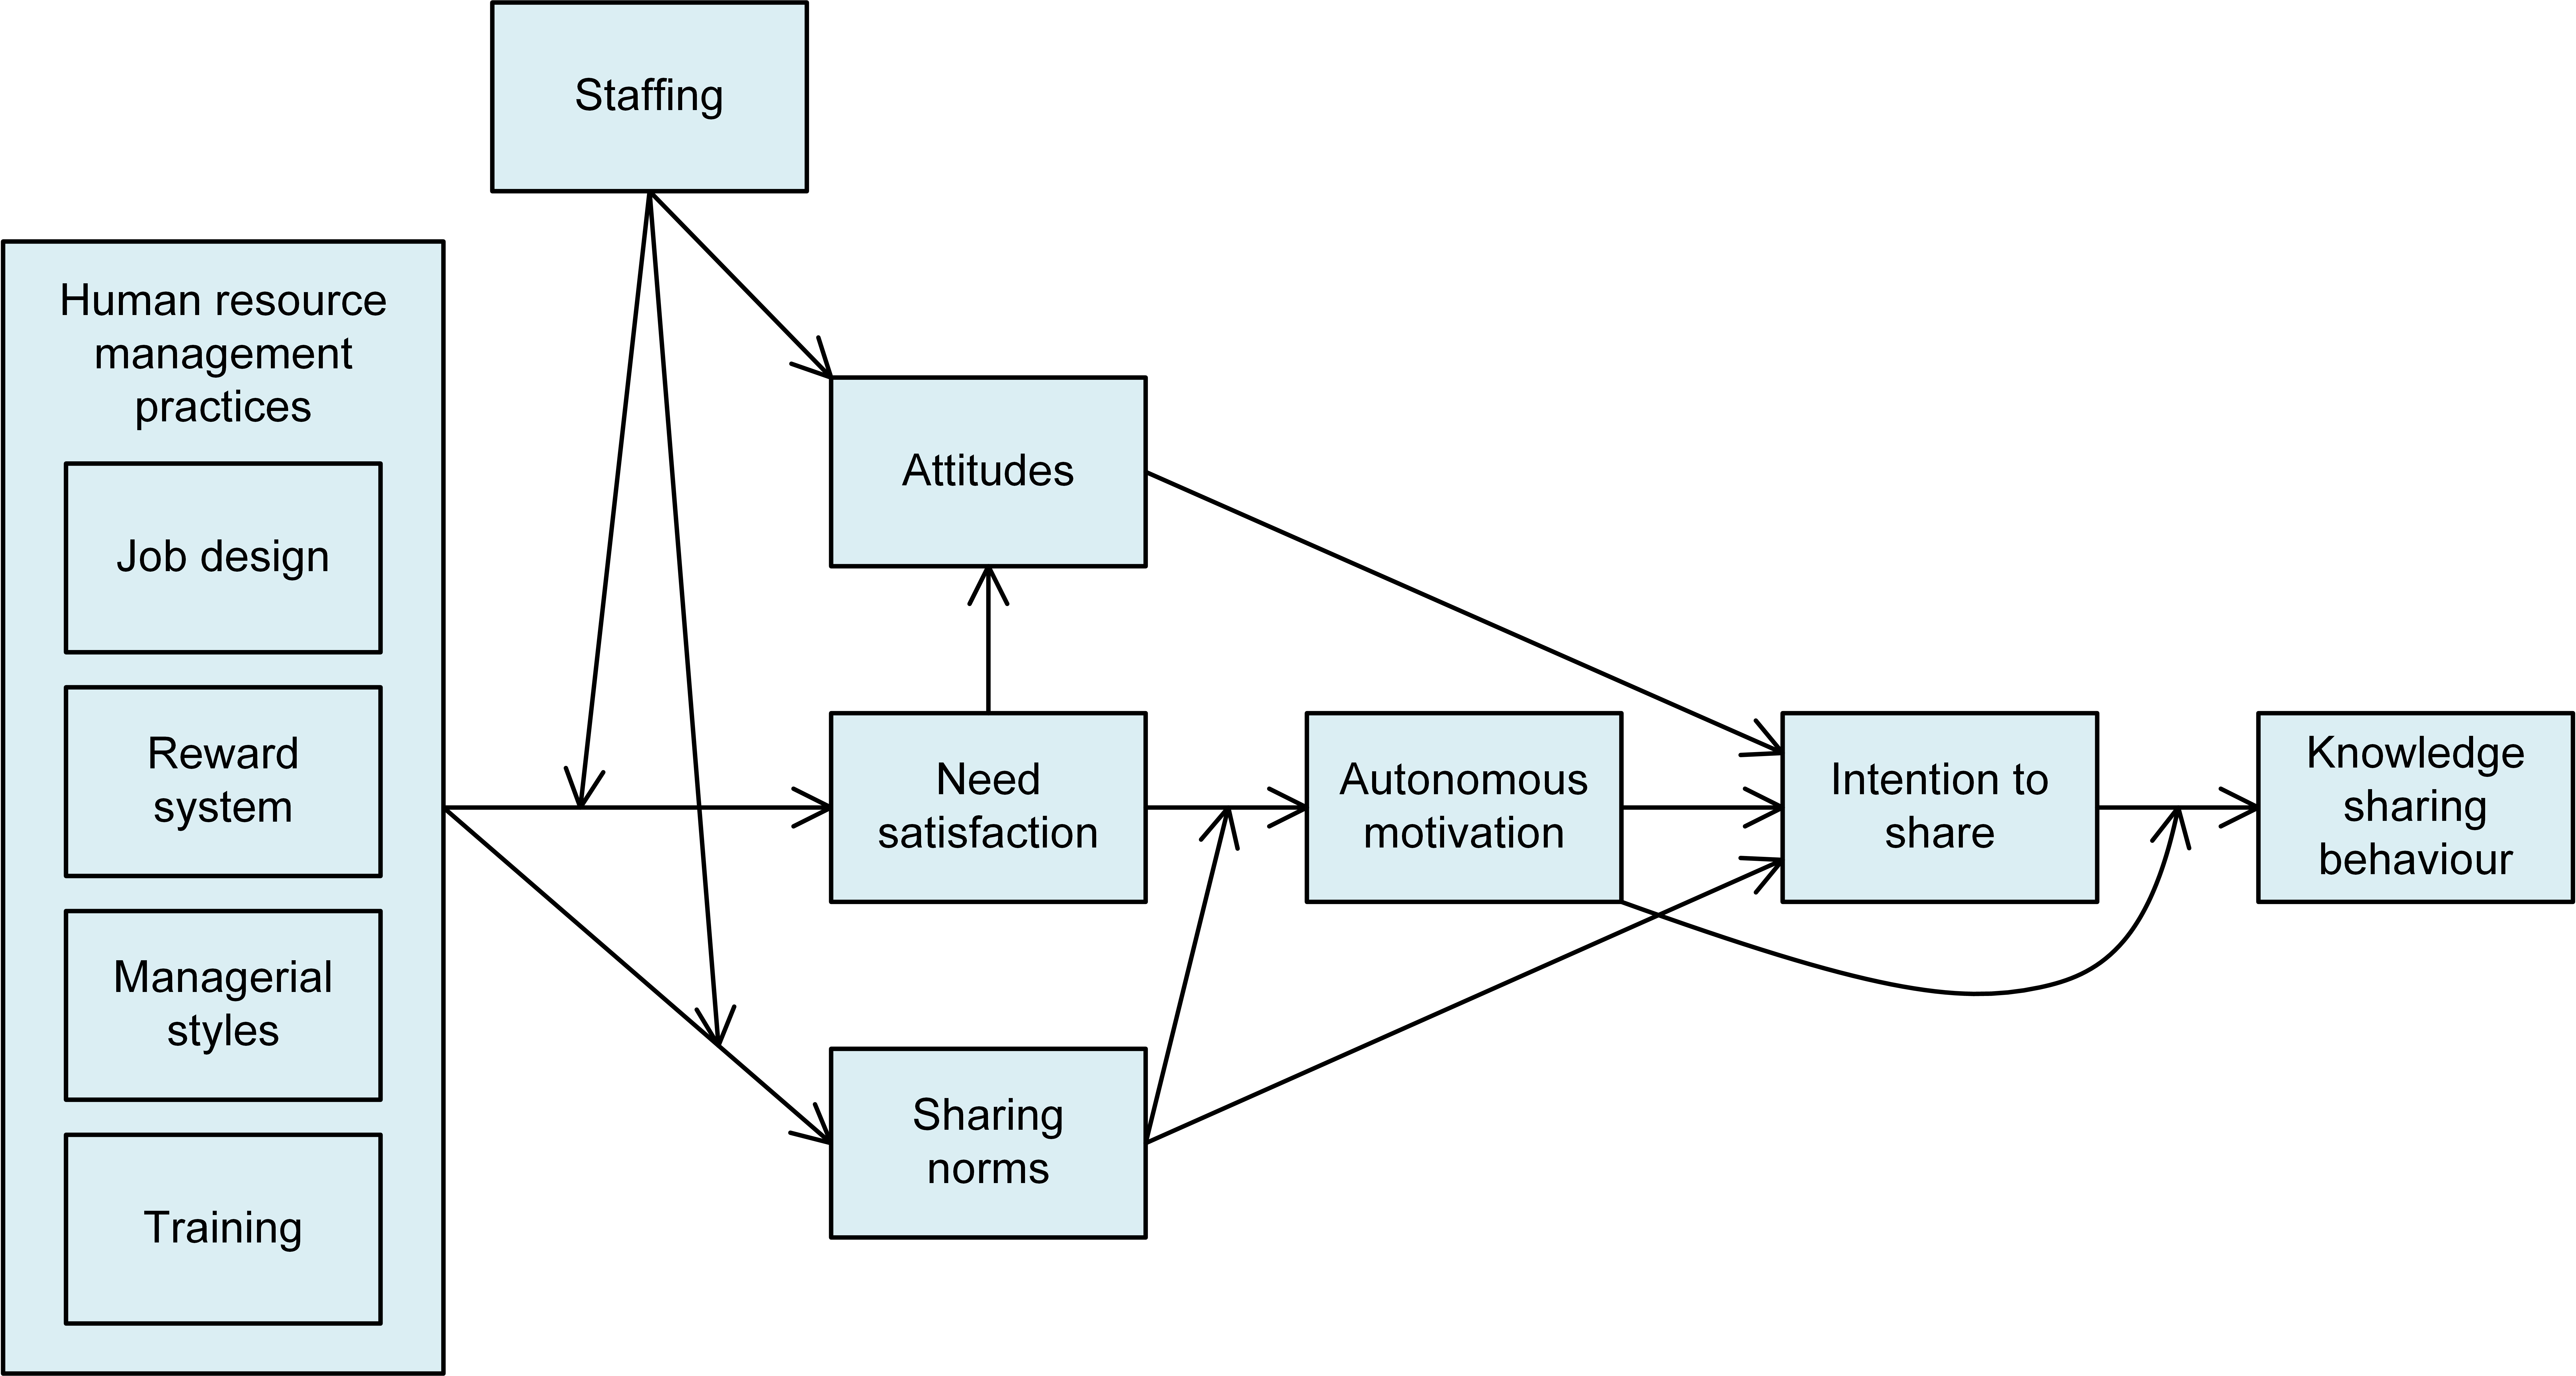
\includegraphics[width=0.9\linewidth]{Images/gagne_model}
	\caption{Model of knowledge sharing motivation \citep{gagne2009model}.}
	\label{fig:gagnemodel}
\end{figure}

A recent study by \citet{llopis2016understanding} examines how a cooperative social climate, intrinsic motivation, and job autonomy influence knowledge sharing behaviour. They suggest the relation between a cooperative climate and knowledge sharing is contingent upon the employee's intrinsic motivation to share knowledge. Results from their survey of employees in a large multinational corporation indicate that people with higher levels of job autonomy are more likely to be influenced by a cooperative climate to share knowledge. More intrinsically motivated people are less likely to be influenced by climate when deciding to share knowledge. \citet{llopis2016understanding} suggest that a cooperative climate can encourage employees who are not intrinsically motivated to share knowledge . \medskip

Most studies examining motivational factors that influence knowledge sharing behaviour do not distinguish between explicit and tacit knowledge. While other studies show that extrinsic rewards do not influence knowledge sharing behaviour in general \citep[e.g.][]{bock2001breaking,bock2005behavioral,lin2007effects}, \citet{hau2013effects} find this is true with respect to tacit knowledge sharing intentions, but not so for explicit knowledge sharing intentions. Their study confirms that reciprocity and enjoyment does influence knowledge sharing intentions more generally. \medskip

Intrinsic motivation is considered crucial for tacit knowledge sharing \citep{osterloh2000motivation}. 

\subsection{Knowledge is power}

Power and knowledge are inextricably intertwined \citep{gaventa2007power}. The current power literature is dominated by two contrasting views of power, namely power as domination, also referred to as power-over, and power as empowerment, often characterised as power-to \citep{haugaard2012rethinking}. 



% power over, power within is seen as repressive
% productive use of power

The network perspective treats power as inherently relational \citep{ibarra1993network}. Power arises from occupying advantageous positions in networks of social relations. The way that an actor is embedded in a social network either imposes constraints on the actor or presents the actor with opportunities. Actors that have fewer constraints and more opportunities than others, occupy favourable structural positions. Being in a favoured position means that an actor may extract better bargains in exchanges, have greater influence, and be a focus for deference and attention from those in less favoured positions \citep{burt1992structural,hanneman2005introduction}. 

There is a co-dependent relationship between power and influence. An actor with power is able to influence others while an actor with influence has power. 

Network centrality measures provide a way to assess how advantageous an actor's position is in a social network. For example, in-degree centrality can be used to measure the number of incoming knowledge ties for each and every actor. High in-degree centrality suggests an actor is empowered because he or she is receiving knowledge from a number of different sources. Burt's measure of constraint measures how much access an actor to network resources \citep{burt1987social}. 




\subsubsection{Personality}

Trait theory is an approach to the study of human personality. Traits define habitual patterns of behaviour, thought, and emotion. They differ across individuals and are stable over time. The \enquote{five-factor model} describes human personality in terms of five traits, namely \enquote{openness to experience}, \enquote{conscientiousness}, \enquote{extraversion}, \enquote{agreeableness}, and \enquote{neuroticism} \citep{mccrae1992introduction}. Table \ref{personality} lists key features of each trait. Essentially, a person's personality can be described in terms of the combined strength of each trait. \medskip 

\begin{landscape}
	\begin{table}[]
		\centering
		\caption{Five-factor model personality traits \citep{mccrae1992introduction,howard1995big}.}
		\label{personality}
		\begin{tabular}{@{}lll@{}}
			\toprule
			Factor & Adjectives & Description \\ \midrule
			Extraversion (E) & \begin{tabular}[c]{@{}l@{}}Active\\ Assertive\\ Energetic\\ Enthusiastic\\ Outgoing\\ Talkative\end{tabular} & Extraversion refers to the number of relationships with which one is comforatble. High extraversion is characterised by a larger number of relationships and a larger proportion of one's time spent in enjoying them. Low extraversion is characterised by a smaller number of relationships and a smaller proportion of one's time spent in pursuing those relationships. \\
			Agreeableness (A) & \begin{tabular}[c]{@{}l@{}}Appreciative\\ Forgiving\\ Generous\\ Kind\\ Sympathetic\\ Trusting\end{tabular} & Agreeableness refers to the number of sources from which one takes one's norms for right behaviour. High agreeableness describes a person who defers to a great many norm sources, such as a spouse, religious leader, friend, boss, or popular culture idol. Low agreeableness describes one who is inclined to only follows one's inner voice. A highly agreeable person will march to the drumbeat of many different drummers, while a less agreeable person marches only to their own drumbeat. \\
			Conscientiousness (C) & \begin{tabular}[c]{@{}l@{}}Capable\\ Organised\\ Resourceful\\ Reliable\\ Responsible\\ Thorough\end{tabular} & Conscientiousness refers to the number of goals on which one is focused. High conscientiousness refers to a person who focuses on fewer goals and exhibits self-discipline associated with such focus. Low conscientiousness refers to one who pursues a larger number of goals and exhibits distractability and spontaneity associated with diffuse focus. \\
			Neuroticism (N) & \begin{tabular}[c]{@{}l@{}}Anxious\\ Self-pitying\\ Tense\\ Touchy\\ Worrying\end{tabular} & Neuroticism is a measure of affect and emotional control. Low levels of neuroticism indicate emotional stability whereas high levels of neuroticism increase the likelihood of experiencing negative emotions. A person with a high level of neuroticism is reactive and more easily bothered by stimuli in their environment. Such a person is prone to becoming unstable,worried, temperamental, and sad. A resistant person, on the other hand, needs strong stimuli to be provoked. \\
			Openness to experience & \begin{tabular}[c]{@{}l@{}}Artistic\\ Curious\\ Imaginative\\ Insightful\\ Original\\ Wide interests\end{tabular} & Openness refers the number of interests to which one is attracted and the depth to which those interests are pursued. High openness refers to a person with relatively more interests and, consequently, relatively less depth within each interest, while low openness refers to a person with relatively few interests and relatively more depth in each of those interests. \\ \bottomrule
		\end{tabular}
	\end{table}
\end{landscape}

Personality has been identified as a factor in knowledge sharing. \citet{matzler2008personality} found agreeableness, conscientiousness and openness to experience are positively correlated with knowledge sharing. People who are conscientious and introverted are more likely to share their tacit knowledge \citep{borges2012tacit}. \citet{stock2014impacts} found those who score higher on openness to experience are more likely to generate new ideas and that being introvert is positively associated with the successful realisation of ideas. They also found those who possess high levels of conscientiousness and neuroticism are more likely to commercially diffuse their innovations. \medskip


\section{Brokerage}

\citet{cohen1990absorptive} see brokers with diverse expertise and contacts playing a key role in the acquisition of knowledge. They believe a diversity of internal perspectives is important to counter resistance towards external knowledge or ideas. \medskip

Brokerage underpins a broad range of organisational phenomena and represents an important mechanism by which intra- and inter-organisational networks evolve and drive change. Brokerage may be conceptualised as a social process that shapes interaction between two or more parties in a wide variety of triadic structures \citep{obstfeld2002knowledge}. Much of the organisational literature dealing with social structures considers brokerage in terms of an open triad, one in which a broker has ties to two alters who are not tied to one another. For example, \citet{marsden1982brokerage} defines brokerage as a mechanism \enquote{by which intermediary actors facilitate transactions between other actors lacking access or trust in one another}.

\citet{fernandez1994dilemma} describe brokerage as a \enquote{relation in which one actor mediates the flow of resources or information between two other actors who are not directly linked}. They argue brokerage \enquote{does not permit the endpoints of a brokerage relation to be directly connected}. \citet{burt1992structural} believes brokers who stand between unconnected alters not only benefit from the novel information that such a structure affords, but are also able to play the disconnected actors against one another. This implies brokerage is more about empowerment of self than about empowering others. \medskip

\citet{obstfeld2014brokerage} describe three strategic orientations to brokerage: \emph{conduit brokerage} is about a third-party who transfers information, knowledge, or other resources between two disconnected parties. The broker mediates rather than moderates the relationship between two others and may help them synthesise new knowledge. With \emph{tertius gaudens brokerage}, the broker aims to exploit differences between two parties by either keeping them apart or playing one against another. In contrast, \emph{tertius iungens brokerage} is about a third-party who introduces two otherwise disconnected parties to each other and encourages them to collaborate (Table \ref{brokerage}). \medskip 

\begin{table}[]
\small
\centering
\caption{Three forms of brokerage process. Reproduced from \citet{obstfeld2014brokerage}.}
\label{brokerage}
\begin{tabularx}{\textwidth}{>{\raggedright}p{3.5cm}>{\raggedright}p{3.5cm}>{\raggedright}p{3.5cm}>{\raggedright}p{3.5cm}}
	\toprule
	& \multicolumn{1}{c}{Conduit} & \multicolumn{1}{c}{Tertius Gaudens} & \multicolumn{1}{c}{Tertius Iungens} \\ 
	\midrule
	& \begin{minipage}{.2\textwidth} \centering 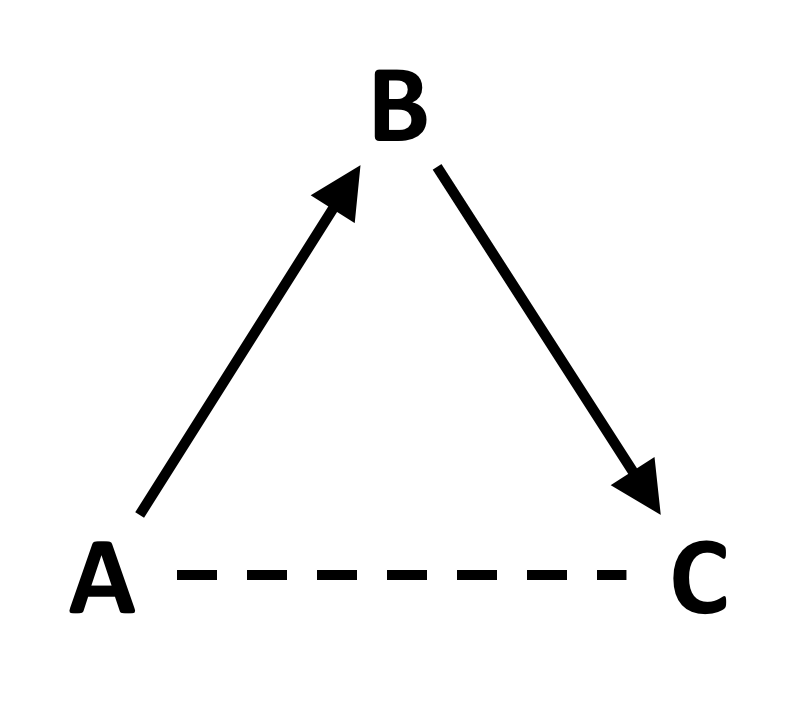
\includegraphics[width=0.7\linewidth]{Images/CDT_brokerage} \end{minipage}  & \begin{minipage}{.2\textwidth} \centering 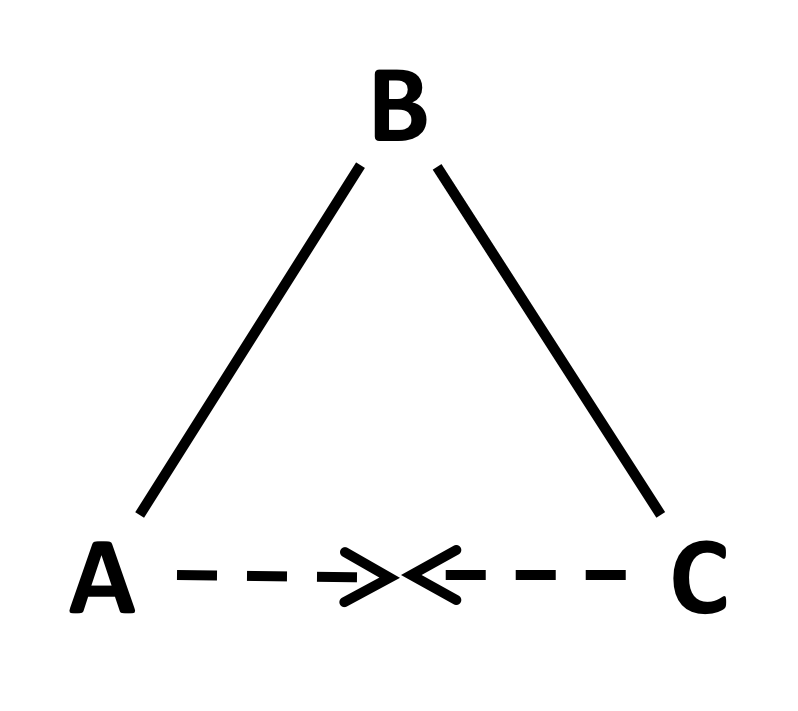
\includegraphics[width=0.7\linewidth]{Images/TG_brokerage_1} \end{minipage}  & \begin{minipage}{.2\textwidth} \centering 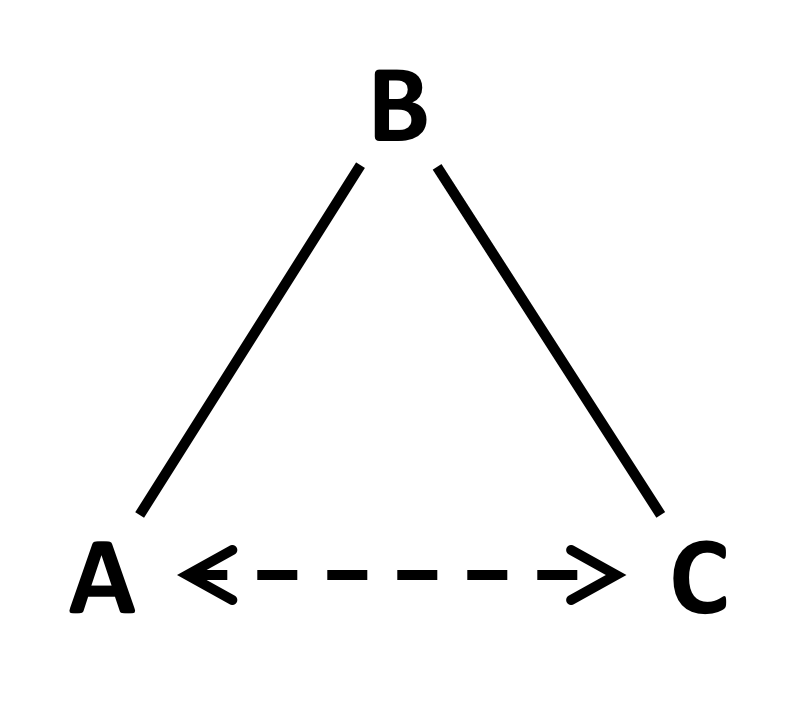
\includegraphics[width=0.7\linewidth]{Images/TI_brokerage} \end{minipage}   \\
	&  &  & \begin{minipage}{.2\textwidth} \centering 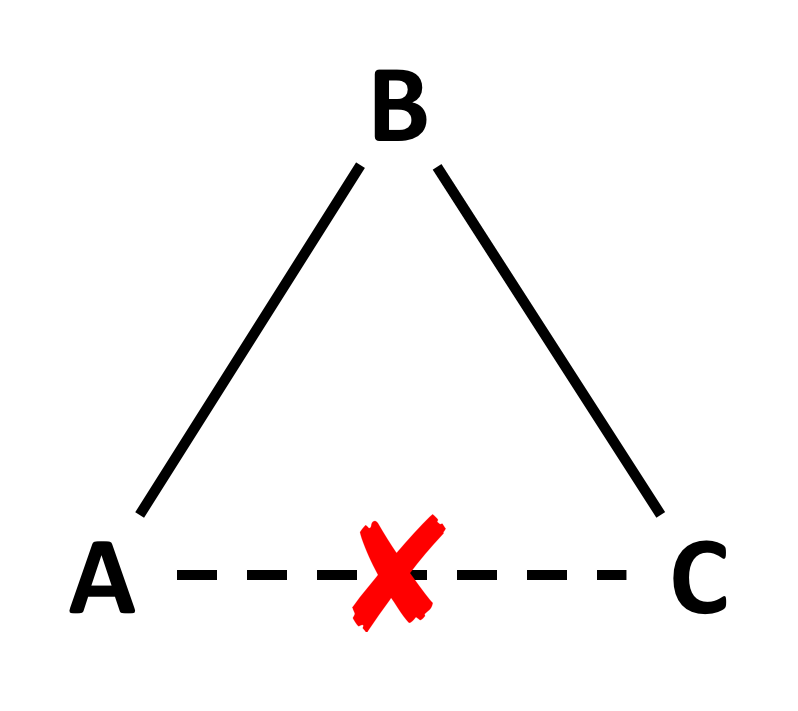
\includegraphics[width=0.7\linewidth]{Images/TG_brokerage_2} \end{minipage}  &  \\
	\midrule
	Open network\\(absence of A-C tie) & B transfers information, knowledge, or other resources between A and C, where A and C have no prospect of meeting. & B plays A and C against one another or keeps A and C apart. & B introduces A and C where A and C have no prior tie. &
	\midrule
	Closed Network\\(presence of A-C tie) & B facilitates transfer between A and C and may help synthesise new knowledge. & B cultivates conflict,competition, or separation between A and C (divide et impera) & B coordinates new collaborative action between A and C. & \\ 
	\bottomrule
\end{tabularx}
\end{table}

With tertius iungens brokerage, a third party introduces or facilitates interaction between two other parties. While tertius gaudens exploits disconnection or negative ties, teritius iungens actively pursues coordination. Tertius iungens brokerage is most opportune when the broker detects opportunities to connect complementary, rather than redundant, alter attributes such as resources and abilities \citep{obstfeld2014brokerage}. Both conduit and iungens draw on knowledge articulation, or the social process by which knowledge is made more explicit, useful, or relevant to the situation at hand \citep{obstfeld2005social,obstfeld2011saying,obstfeld2012creative}.

From an open innovation perspective, \emph{tertius iungens} brokerage is quite important, especially in the early stages of collaboration, when many actors do not know fellow collaborators in partner organisations. Not only that, knowledge held by third parties is also likely to be unfamiliar. Once ties have been established through \emph{tertius iungens} brokerage, \emph{conduit} brokerage is needed to help synthesise and transform knowledge into novel ideas \citep{fleming2007collaborative,lingo2010nexus,quintane2016brokers}. \citet{gould1989structures} describe \emph{conduit} brokerage in terms of \emph{coordination}, \emph{liaison}, \emph{itinerant}, \emph{representative}, and \emph{gatekeeper} roles (Table \ref{gf_params}). Each role expresses a different power dynamic and one should be able to use the relative proportion of each role to characterise power-relations in open innovation collaborations. \medskip

\begin{table}[]
	\small
	\centering
	\caption{Gould-Fernandez brokerage roles. After \citet{gould1989structures} and \citet{butts2016package}.}
	\label{gf_params}
	\begin{tabularx}{\textwidth}{@{}lcl@{}}
		\toprule
		\multicolumn{1}{c}{Role} & \multicolumn{1}{c}{Motif} & \multicolumn{1}{c}{Explanation} \\ \midrule
		Liaison (b\textsubscript{O})			&  \begin{minipage}{.2\textwidth} \centering 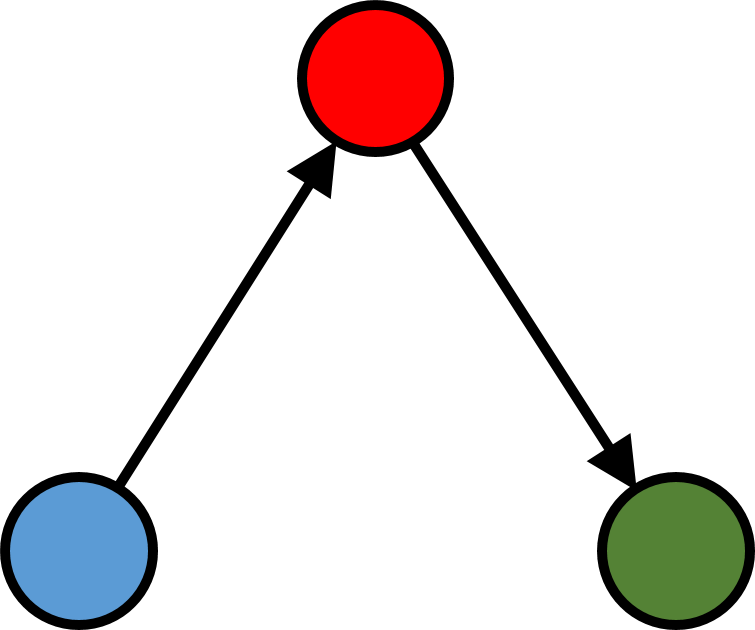
\includegraphics[width=0.4\linewidth]{Images/b_O} \end{minipage}	& \begin{tabular}[c]{l}Broker mediates contact between two\\ individuals from different groups,\\ neither of which is the group to\\ which he or she belongs.\end{tabular}\\ [10ex]
		Representative  (b\textsubscript{IO})	& \begin{minipage}{.2\textwidth} \centering 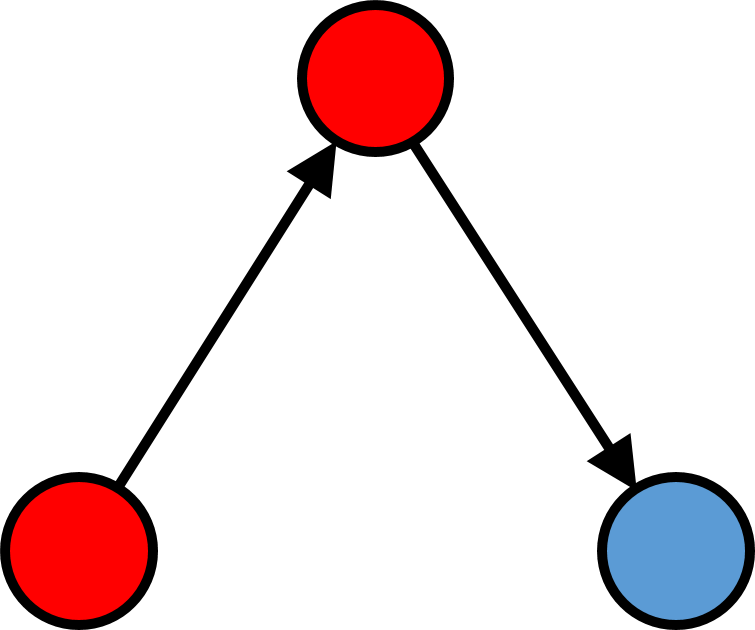
\includegraphics[width=0.4\linewidth]{Images/b_IO} \end{minipage}   & \begin{tabular}[c]{l}Broker mediates an outgoing contact\\ from an in-group member to an\\ out-group member.\end{tabular}\\ [10ex]
		Gatekeeper (b\textsubscript{OI})		& \begin{minipage}{.2\textwidth} \centering 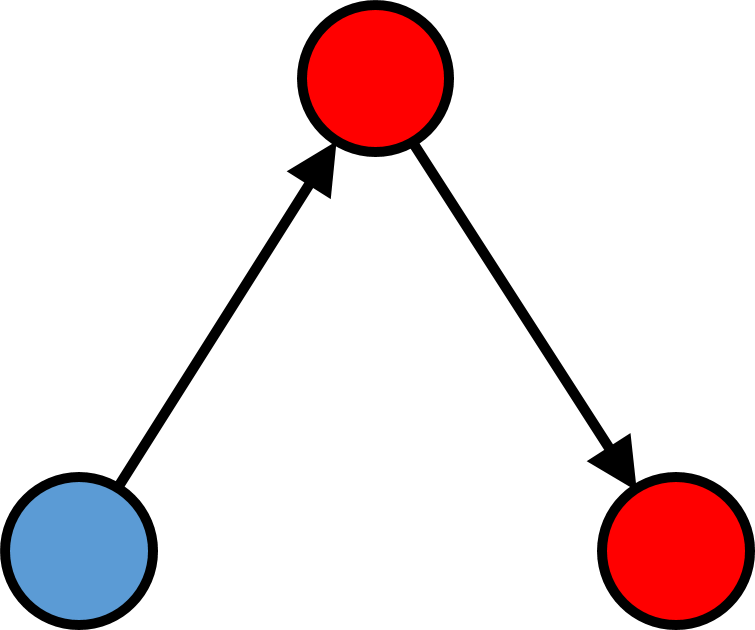
\includegraphics[width=0.4\linewidth]{Images/b_OI} \end{minipage}   & \begin{tabular}[c]{l}Broker mediates an incoming contact\\ from an out-group member to an\\ in-group member. \end{tabular}\\ [10ex]
		Itinerant broker (w\textsubscript{O})	&  \begin{minipage}{.2\textwidth} \centering 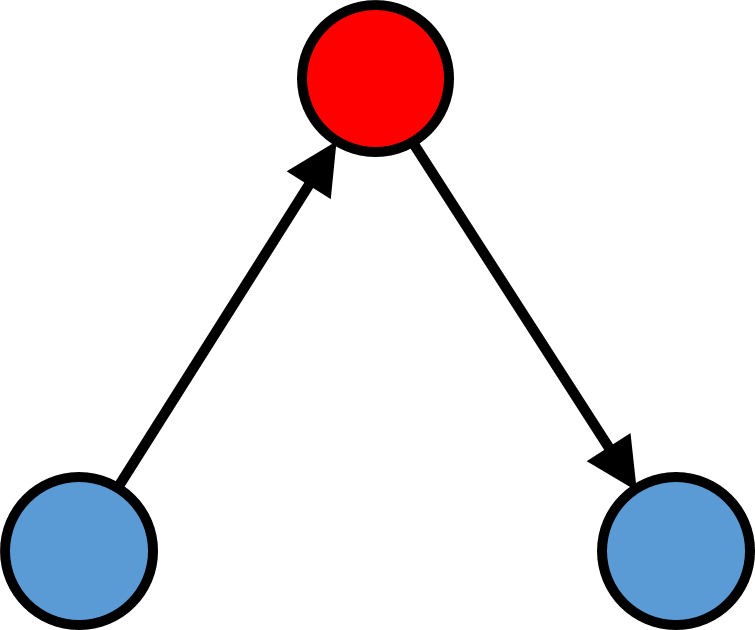
\includegraphics[width=0.4\linewidth]{Images/w_O} \end{minipage}   & \begin{tabular}[c]{l}Broker mediates contact between two\\ individuals from a single group to\\ which he or she does not belong. \end{tabular}\\ [10ex]
		Coordination (w\textsubscript{I})		& \begin{minipage}{.2\textwidth} \centering 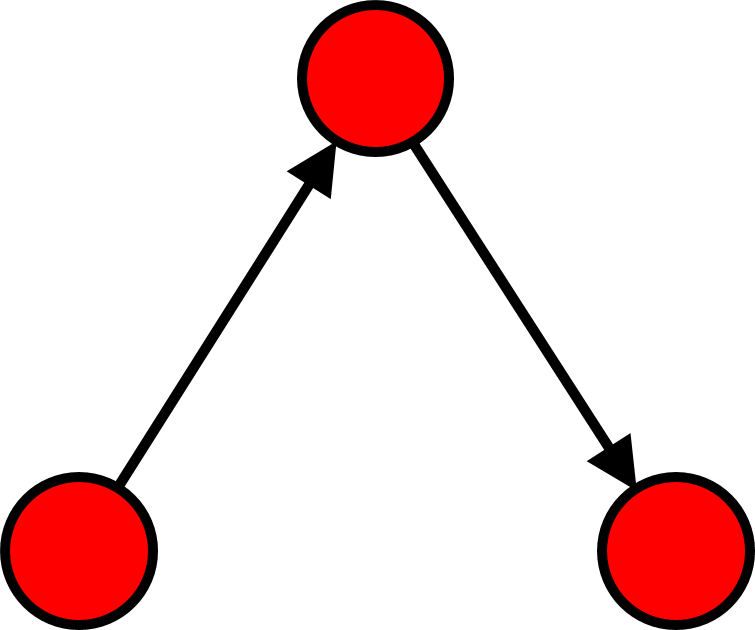
\includegraphics[width=0.4\linewidth]{Images/w_I} \end{minipage}    & \begin{tabular}[c]{l}Broker mediates contact between two\\ individuals from his or her own\\ group. \end{tabular}\\ 
		\bottomrule
	\end{tabularx}
\end{table}

Effective brokerage strategies may require complex combinations and sequences of different brokerage behaviours over time. Skilled brokerage often involves selective deployment of these approaches with different actors or for different objectives. Different combinations of tertius iungens and tertius gaudens behavior are necessary to tailor brokerage strategies to match the situation \citep{obstfeld2014brokerage}. ... Davis’s (2011) study of innovative alliances in the computer industry found that active pruning of old ties may be necessary before man- agers can effectively facilitate new ties, suggesting that sequences of gaudens and iungens behavior are sometimes necessary.

\section{Defining innovation}

This study defines innovation as \enquote{the development and implementation of new ideas by people who, over time, engage in relationships with others within an institutional and environmental context} \citep{van1986central}. So long an idea is perceived as new to the people involved, it should be seen as an innovation even though others may view it as an imitation of something that exists elsewhere \citep{van1986central}. From a business perspective, innovation is about renewal of the enterprise so it can enhance its ability to create value and remain competitive \citep{schumpeter1950capitalism}. Failure to innovate places a firm's ability to survive and prosper at risk \citep{bessant2005managing}. \medskip 

\section{The multifaceted nature of knowledge}


\section{Sources of competitive advantage}

According to the resource-based view of the firm, competitive advantage stems from the application of tangible and intangible resources available to the firm \citep{wernerfelt1984resource,peteraf1993cornerstones}. Sustained competitive advantage can be achieved if these resources are valuable, rare, inimitable, and non-substitutable \citep{barney1991firm}. A derivative of the resource-based view is the knowledge-based view of the firm, which considers knowledge to be the most important resource of a firm \citep{grant1996toward}. The knowledge-based view emphasises the importance of having effective processes for transferring knowledge across organisational boundaries \citep{kogut1992knowledge,grant1996toward}. This requires a relational view that focuses on the social structures, routines, and processes for knowledge exchange \citep{dyer1998relational,nahapiet1998social}. Open innovation substantiates the relational view of competitive advantage. The business model that underpins open innovation explains how relational rents can be generated from knowledge sharing activities \citep{durst2013success}. \medskip

Transforming the existing business model to support open innovation, changing internal approaches to research and development, building a more open culture, finding appropriate organisations to partner with, and protecting intellectual property are some of the more pressing challenges \citep{dahlander2010open,sieg2010managerial,lichtenthaler2011your,durst2013success,roper2013externalities,aloini2016structured}. 

While tacit knowledge can play a key role in overcoming relative differences in absorptive capacity, mobilising tacit knowledge is a challenge in itself \citep{gassmann2004towards,bahemia2010contingent,bogers2011open}. More on the challenges of overcoming absorptive capacity and mobilising tacit knowledge below. \medskip

\subsubsection{Relative differences in absorptive capacity}


 
Despite a vast body of research that has examined various aspects of absorptive capacity, the concept remains elusive for both researchers and practitioners \citep{duchek2013capturing,omidvar2013revisiting}. Early conceptualisations of absorptive capacity emphasised the importance of prior related knowledge to help bridge cognitive gaps \citep{cohen1989innovation,cohen1990absorptive}. These early conceptualisations paid little attention to the processes that build absorptive capacity \citep{zahra2002absorptive}. More recent conceptualisations treat absorptive capacity as a dynamic capability\footnote{Ordinary capabilities encapsulate the core business functions of operations, administration, and governance. Dynamic capabilities, on the other hand, refer to the firm's capacity to sense new opportunities, mobilise resources to take advantage of opportunities, and maintaining competitiveness through enhancing, protecting and configuring its tangible and intangible resources \citep{teece2007explicating,teece2014foundations}.} that integrates processes for acquiring, assimilating, transforming, exploiting new knowledge \citep{zahra2002absorptive,lane2006reification,todorova2007absorptive,volberda2010perspective,lewin2011microfoundations,marabelli2014knowing}. Absorptive capacity may be viewed as a form of organisational learning addressing new external knowledge, one that involves processes and routines to share, communicate, and transfer individual learning to the group and organisational levels \citep{sun2010examination}. \medskip

Building absorptive capacity is challenging because it cuts across multiple levels and is contingent not only on prior related knowledge and social mechanisms for integrating diverse knowledge, but also on the strength or weakness of appropriability regimes \footnote{The term \enquote{appropriability regime} refers to the extent to which knowledge and innovations can be protected from imitators \citep{teece1998capturing,hurmelinna2007nature}.} and nature of power-relations \citep{todorova2007absorptive,easterby2008absorptive,duchek2013capturing}. \medskip 

Knowledge is something that exists on a spectrum where at one extreme, it is almost completely tacit, that is knowledge held in peoples' minds and bodies. At the other extreme, knowledge is almost completely explicit, existing in codified or structured form and accessible to other people \citep{polanyi1966tacit,inkpen1998knowledge,leonard1998role,cavusgil2003tacit}.  

Another way to facilitate the transfer of tacit knowledge is through communities of practice \citep{lave1991situated,brown2001knowledge,smith2001role,cox2005communities,easterby2008inter}. These function as a social instrument to create, share and steward knowledge, and are a pragmatic basis of an organisation’s absorptive capacity and significant sites of innovation \citep{brown1991organizational}. \medskip





%The literature chapter might pick up from the introduction of the research focus and why it is a significant area of inquiry. Thus the issue of collaborative practice and  knowledge-sharing in the contemporary innovation and creativity policy and business environment might be worthwhile mentioning as background. These seem to fit in well with your propositions under literature review
 
%The wide base of the pyramid then narrows to the role that open innovation has been seen as playing in this environment. My choice would be to discuss social capital building as a form of competitive advantage drawing from Nahapiet and Ghoshal's work. This also allows the introduction of collaboration and power through knowledge creation at a macro and micro level and fits well with the more critical appraisal of N & G. This area might be expanded when you produce the first draft.

%This issue of power and knowledge creation, transfer could provide a link with motivation as a key concept from the perspective of exploring intrinsic/extrinsic motivation i.e. what are the boundaries or limits of extrinsic motivation in dynamic and contextual situations. This allows your critique of Gagne's work that in organisations knowledge sharing behaviour can be explained in terms of TPB/SDT [Gagne 2009]. The feedback to date suggests we might want to discuss further the contribution of TPB theory in the context in which you want to explore it, but I think, as you define it below, it has a place in framing issues apparently highlighted within your data.

%Finally, the role of brokerage also appears to be conceptually synergistic with power wileding in knowledge sharing and open innovation, so I like your 3rd proposition.

%You  also seem to be suggesting that your findings will identify certain skillsets, approaches and behaviours that appear to have value in effective open innovation (from the perspectives of your subjects when interviewed) and which might highlight useful approaches in given contexts (stages of the project and characteristics and stakes of stakeholders being factors worth considering).

%So I think that you have a good framework here which we can refine as your analysis and findings become clearer and we can identify any conceptual issues that might need raising either upfront in your literature review or in the context of your discussion of findings and further research.


 


Relative differences in absorptive capacity can impede the flow of knowledge across organisational boundaries, create power imbalances, and undermine alliance performance.  
- Need to recognise knowledge is a form of power.
- Useful to understand how knowledge sharing behaviour is influenced by personal motivation, power-relations, and organisational factors.
 
\section{Characterising tacit knowledge} 

- Very hard to describe tacit knowledge. 
- Not possible to measure directly
- Indirect approaches.

\section{Knowledge is power}

 
\section{Motivation to share knowledge}
 
- What is motivation? Motivation is a theoretical construct used to explain behaviour.
- people are motivated to share knowledge either out of self-interest, altruism, or both. [Hsiu-Fen Lin, 2007]
- people motivated out of self-interest do so to empower themselves in two ways - satisfy some innate need or gain some personal advantage by being gatekeeper of knowledge.
- people motivated out of altruism want everybody, including themselves, to succeed. They succeed if everybody else succeeds.
- we can look at motivation in terms of self-determination theory (innate needs) and brokerage (behaviour, actions).
- Tacit knowledge requires more effort (i.e. higher levels of motivation) to communicate.  [osterloh and frey 2000]
- Past studies show that intrinsic motivation predicts tacit knowledge sharing e.g.
 
\subsection{Self-determination theory}
 
 
- Many motivational theories. With innovation, interested on motivation for learning.
- Innovation is intrinsically motivated. [Bhaduri & Kumar 2011]
- SDT is useful for assessing intrinsic and extrinsic motivation.
- SDT argues behaviour is driven by innate need for competence, autonomy and relatedness.
- SDT conceptualise motivation as a continuum comprising amotivation, extrinsic motivations, and intrinsic motivation.
- SDT suggest extrinsic motivations differ depending on locus of control.
- Material and introjected regulation locus is external. Integrated and identified regulation locus is internal.
- Intrinsic motivation is by definition internal.
- The more one internalises reasons for externally motivated actions, the more these actions become self-determined.
- Knowledge sharing behaviour can be explained in terms of TPB/SDT [Gagne 2009]
- TPB explains how attitudes, norms may influence externally regulated behaviour (extrinsic motivators).
 
\emph{Proposition 1A: People with higher levels of autonomous motivation are more likely to share tacit knowledge.}

\emph{Proposition 1B: People with higher levels of autonomous motivation are more likely to seek out tacit knowledge.}
 
 
\section{Brokerage}
 
- Define brokerage [ Marsden 1982 ]
- Brokerage roles [ Gould and Fernandez 1989]
- Strategic orientations - tertius gaudens [Burt] vs, tertius inungens [Obstfeld]
- Knowledge is power. Consider brokerage in terms of self-empowerment vs. empowering others [ soda, tortoriello, iorio 2017 ]
- Brokers in innovation networks
 
\emph{Proposition 3: Power in open innovation collaborations can be characterised in terms of brokerage roles.}
 
\section{Summary}
 
- Large part of managing knowledge flows in open innovation is about creating a climate conducive to knowledge sharing.
- Cannot coerce people to share knowledge - this is something that must be done through volition.
- Understanding what motivates people to share and/or broker knowledge is a good first step.
- TPB and SDT can help with this.
- Also important to consider knowledge as power.
- Next section explains how mixed method SNA can be used to assess knowledge sharing/brokerage behaviour and power relations. 